\documentclass[11pt, oneside]{article}   	% use "amsart" instead of "article" for AMSLaTeX format
\usepackage{geometry}                		% See geometry.pdf to learn the layout options. There are lots.
\geometry{letterpaper}                   		% ... or a4paper or a5paper or ... 
%\geometry{landscape}                		% Activate for for rotated page geometry
%\usepackage[parfill]{parskip}    		% Activate to begin paragraphs with an empty line rather than an indent
\usepackage{graphicx}				% Use pdf, png, jpg, or eps� with pdflatex; use eps in DVI mode
								% TeX will automatically convert eps --> pdf in pdflatex		
\usepackage{amssymb}
\usepackage{amsmath}
\usepackage{parskip}
\usepackage{color}
\usepackage{hyperref}

\title{Integrate the square root of z}
%\author{The Author}
%\section{}
%\subsection*{}
\date{}							% Activate to display a given date or no date

\graphicspath{{/Users/telliott_admin/Dropbox/Tex/png/}}
% \begin{center} 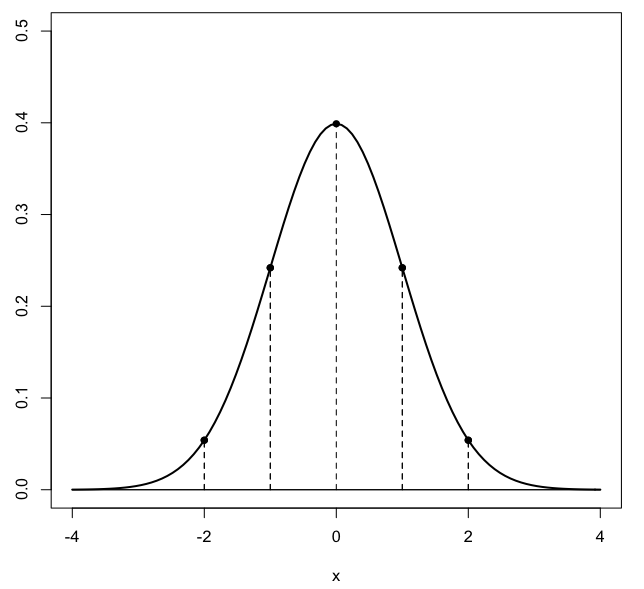
\includegraphics [scale=0.4] {gauss3.png} \end{center}
\begin{document}
\maketitle
\Large
Consider
\[ \int \sqrt{z} \ dz \]
along the half-circle of radius $3$ starting from the point $z = R$ on the $x$-axis and proceeding counter-clockwise.
We can do this integral even if the "branch" of the square root function that we're using is only defined for $\theta > 0$.  We have that 
\[ z = Re^{i\theta}, \ \ \ \theta = 0 \rightarrow \pi \]
\[ dz = iz = iRe^{i\theta} \ d \theta \]
\[ \sqrt{z} = \sqrt{R} e^{i\theta/2} \]
so
\[ I = \int_0^{\pi} iR \sqrt{R} e^{i3\theta/2} \ d \theta \]
We need
\[ \int e^{i3\theta/2} \ d \theta = \frac{2}{3i} e^{i3\theta/2} \ \bigg |_0^{\pi} \]
easiest to write it out as
\[ e^{i3\theta/2} \ \bigg |_0^{\pi} = \cos \frac{3\pi}{2} + i \sin  \frac{3\pi}{2} - \cos 0 - i \sin 0 \]
\[ = 0 + i(-1) - 1 - 0 = -(1+i) \]
Going back to pick up all the factors we left behind:
\[ I = -iR \sqrt{R} \ \frac{2}{3i} \ (1+i) = -R \sqrt{R} \ \frac{2}{3} \ (1+i) \]
In the problem, $R$ was actually specified as $3$, leading to the cancellation:
\[ I = - 2 \sqrt{3} \ (1+i) \]

We can also do this problem by antiderivatives:
\[ \int_R^{-R} \sqrt{z} \ dz = \frac{2}{3} \ z^{3/2} \ \bigg |_R^{-R}  \]
\[ = \frac{2}{3} ( R^{3/2} e^{i3\pi/2} - R^{3/2} e^0) \]
\[ = \frac{2}{3} R^{3/2} ( e^{i3\pi/2} - 1) \]
and, as we showed above:
\[ e^{i3\pi/2} = -i \]
If $R=3$ we get the same answer as before.

\end{document}  